\PassOptionsToPackage{unicode=true}{hyperref} % options for packages loaded elsewhere
\PassOptionsToPackage{hyphens}{url}
\documentclass[11pt,dvipsnames,ignorenonframetext,aspectratio=169]{beamer}
\IfFileExists{pgfpages.sty}{\usepackage{pgfpages}}{}
\setbeamertemplate{caption}[numbered]
\setbeamertemplate{caption label separator}{: }
\setbeamercolor{caption name}{fg=normal text.fg}
\beamertemplatenavigationsymbolsempty
\usepackage{lmodern}
\usepackage{amssymb,amsmath}
\usepackage{ifxetex,ifluatex}
\usepackage{fixltx2e} % provides \textsubscript
\ifnum 0\ifxetex 1\fi\ifluatex 1\fi=0 % if pdftex
  \usepackage[T1]{fontenc}
  \usepackage[utf8]{inputenc}
\else % if luatex or xelatex
  \ifxetex
    \usepackage{mathspec}
  \else
    \usepackage{fontspec}
\fi
\defaultfontfeatures{Ligatures=TeX,Scale=MatchLowercase}







\fi

  \usetheme[]{monash}

  \usecolortheme{monashwhite}


% A default size of 24 is set in beamerthememonash.sty

% Title page
\setbeamertemplate{title page}
{\placefig{-0.01}{-0.01}{width=1.01\paperwidth,height=1.01\paperheight}{solitary\_mushroom.jpg}
\begin{textblock}{7.5}(1,2.8)\usebeamerfont{title}
{\color{white}\raggedright\par\inserttitle}
\end{textblock}
\begin{textblock}{7.5}(1,7)
{\color{white}\raggedright{\insertauthor}\mbox{}\\[0.2cm]
\insertdate}
\end{textblock}}


  \useinnertheme{rounded}

  \useoutertheme{smoothtree}

% use upquote if available, for straight quotes in verbatim environments
\IfFileExists{upquote.sty}{\usepackage{upquote}}{}
% use microtype if available
\IfFileExists{microtype.sty}{%
  \usepackage{microtype}
  \UseMicrotypeSet[protrusion]{basicmath} % disable protrusion for tt fonts
}{}


\newif\ifbibliography
  \usepackage[round]{natbib}
  \bibliographystyle{plainnat}


\hypersetup{
      pdftitle={Stage of development, application of natural enemies, composition of innoculums and evaluation aspects},
            colorlinks=true,
    linkcolor=red,
    citecolor=Blue,
    urlcolor=lightgrayd,
    breaklinks=true}
%\urlstyle{same}  % Use monospace font for urls







% Prevent slide breaks in the middle of a paragraph:
\widowpenalties 1 10000
\raggedbottom

  \AtBeginPart{
    \let\insertpartnumber\relax
    \let\partname\relax
    \frame{\partpage}
  }
  \AtBeginSection{
    \ifbibliography
    \else
      \let\insertsectionnumber\relax
      \let\sectionname\relax
      \frame{\sectionpage}
    \fi
  }
  \AtBeginSubsection{
    \let\insertsubsectionnumber\relax
    \let\subsectionname\relax
    \frame{\subsectionpage}
  }



\setlength{\parindent}{0pt}
\setlength{\parskip}{6pt plus 2pt minus 1pt}
\setlength{\emergencystretch}{3em}  % prevent overfull lines
\providecommand{\tightlist}{%
  \setlength{\itemsep}{0pt}\setlength{\parskip}{0pt}}

  \setcounter{secnumdepth}{0}


%% Monash overrides
\AtBeginSection[]{
   \frame<beamer>{
   \frametitle{Outline}\vspace*{0.2cm}
   
   \tableofcontents[currentsection,hideallsubsections]
  }}

% Redefine shaded environment if it exists (to ensure text is black)
\ifcsname Shaded\endcsname
  \definecolor{shadecolor}{RGB}{225,225,225}
  \renewenvironment{Shaded}{\color{black}\begin{snugshade}\color{black}}{\end{snugshade}}
\fi
%%


  \usepackage{setspace}
  \usepackage{wasysym}
  % \usepackage{footnote} % don't use this this breaks all
  \usepackage{fontenc}
  \usepackage{fontawesome}
  \usepackage{booktabs,siunitx}
  \usepackage{longtable}
  \usepackage{array}
  \usepackage{multirow}
  \usepackage{wrapfig}
  \usepackage{float}
  \usepackage{colortbl}
  \usepackage{pdflscape}
  \usepackage{tabu}
  \usepackage{threeparttable}
  \usepackage{threeparttablex}
  \usepackage[normalem]{ulem}
  \usepackage{makecell}
  \usepackage{xcolor}
  \usepackage{tikz} % required for image opacity change
  \usepackage[absolute,overlay]{textpos} % for text formatting
  \usepackage{chemfig}
  \usepackage[skip=0.333\baselineskip]{caption}
  % \newcommand*{\AlignChar}[1]{\makebox[1ex][c]{\ensuremath{\scriptstyle#1}}}%
  \usepackage{siunitx}

  % this font option is amenable for beamer
  \setbeamerfont{caption}{size=\tiny}
  \singlespacing
  \definecolor{lightgrayd}{gray}{0.95}
  \definecolor{skyblued}{rgb}{0.65, 0.6, 0.94}
  \definecolor{oranged}{RGB}{245, 145, 200}

  % % better to insert it into template itself
  % \newlength{\cslhangindent}
  % \setlength{\cslhangindent}{1.5em}
  % \newenvironment{cslreferences}%
  %   {\setlength{\parindent}{0pt}%
  %   \everypar{\setlength{\hangindent}{\cslhangindent}}\ignorespaces}%
  %   {\par}

  \usepackage[caption=false]{subfig}

  \newcommand{\bcolumns}{\begin{columns}[T, onlytextwidth]}
  \newcommand{\ecolumns}{\end{columns}}

  \newcommand{\bdescription}{\begin{description}}
  \newcommand{\edescription}{\end{description}}

  \newcommand{\bitemize}{\begin{itemize}}
  \newcommand{\eitemize}{\end{itemize}}
  \AtBeginSubsection{}

  \title[]{Stage of development, application of natural enemies,
composition of innoculums and evaluation aspects}


  \author[
        \vspace{-0.5cm}Deependra Dhakal\\
Assistant Professor\\
Agriculture and Forestry University\\
\textit{ddhakal.rookie@gmail.com}\\
\url{https://rookie.rbind.io}
    ]{\vspace{-0.5cm}Deependra Dhakal\\
Assistant Professor\\
Agriculture and Forestry University\\
\textit{ddhakal.rookie@gmail.com}\\
\url{https://rookie.rbind.io}}


\date[
      
  ]{
    }

\begin{document}

% Hide progress bar and footline on titlepage
  \begin{frame}[plain]
  \titlepage
  \end{frame}


   \frame<beamer>{
   \frametitle{Outline}\vspace*{0.2cm}
   
   \tableofcontents[hideallsubsections]
  }

\hypertarget{host-stage-of-development-for-testing-and-application-of-natural-enemy}{%
\section{(Host) Stage of development for testing and application of
natural
enemy}\label{host-stage-of-development-for-testing-and-application-of-natural-enemy}}

\begin{frame}{Seedling versus mature plants}
\protect\hypertarget{seedling-versus-mature-plants}{}
\begin{itemize}
\tightlist
\item
  Hypersensitive response of a host genotype during seedling stages is
  more pronounced, although the resistance type is effective even in the
  mature plants. Mature plants also express a greater number of
  hypersensitivity genes, in contrast.
\item
  Obvious advantage of seedling tests are:

  \begin{itemize}
  \tightlist
  \item
    require less space
  \item
    can be performed soon after growing
  \item
    be inoculated more uniformly than large, mature plants
  \item
    fairly uniform in their growth in early stages of development
  \end{itemize}
\end{itemize}
\end{frame}

\begin{frame}{}
\protect\hypertarget{section}{}
\begin{itemize}
\tightlist
\item
  Partial resistance is less pronounced in seedling than in later stages
  of the plant development, for example, in biotrophic fungi (rusts,
  smuts and powdery mildew fungi).

  \begin{itemize}
  \tightlist
  \item
    in laboratory tests for level of resistance or susceptibility
    against \emph{Septoria nodorum} pathogen mature plants have to be
    used, such that inoculation of wheat is carried out after the
    complete formation of the third leaf.
  \item
    effectiveness of genes for partial resistance are probably partly
    dependent on the stage of the development of plant
  \item
    in natural enemies specialized to live on fruits, flower and stem,
    tests are usually carried out in the field on mature plants
  \end{itemize}
\item
  Detached plant parts such as leaf disks, entire leaves or branches of
  trees may be tested for resistance by exposing them to natural enemy
  (usually under controlled conditions)
\end{itemize}
\end{frame}

\begin{frame}{Stage of plant inoculation (case with virus)}
\protect\hypertarget{stage-of-plant-inoculation-case-with-virus}{}
\begin{table}

\caption{\label{tab:plant-specis-inoculum-stage}Commonly used test plant species, with their age, and stage of development (number and/or type of leaves) suitable for inoculation.}
\centering
\fontsize{6}{8}\selectfont
\begin{tabular}[t]{>{\raggedright\arraybackslash}p{15em}>{\raggedright\arraybackslash}p{8em}>{\raggedright\arraybackslash}p{14em}}
\toprule
Species/cultivar & Age (days) & Stage of development\\
\midrule
\textit{Beta vulgaris} & 20-25 & 2\\
\textit{Capsicum annum} & 35 & 3\\
\textit{Chenopodium} spp. & 28 & 3-4 well-developed\\
\textit{Cucumis sativus} & 10 & Cotyledons\\
\textit{Glycine max} & 14 & Cotyledons+1\\
\addlinespace
\textit{Gomphrena globosa} (Makhamali) & 40-50 & 2-3 pairs\\
\textit{Helianthus annus} & 16 & 1 pair\\
\textit{Lycopersicon esculentum} & 21-28 & 2-3\\
\textit{Nicotiana tabacum} & 28-30 & 2 well-developed\\
\textit{Petunia hybrida} & 29 & 3 well-developed\\
\addlinespace
\textit{Phaseolus vulgaris} & 10 & 2 primary\\
\textit{Pisum sativum} & 13 & 2\\
\textit{Solanum melongena} & 30 & 2\\
\textit{Vicia faba} & 14 & 1\\
\textit{Vigna unguiculata} & 10 & 2 primary\\
\bottomrule
\end{tabular}
\end{table}
\end{frame}

\begin{frame}{Applying natural enemy}
\protect\hypertarget{applying-natural-enemy}{}
\begin{itemize}
\tightlist
\item
  Important consideration is that each plant (part) is exposed to same
  amount of inoculum (per \si{\square\centi\meter}, per fruit)
\item
  Variation in degree of infection between plants should not be result
  of escape or differences in density of inoculation.
\item
  General methods of application comprise

  \begin{itemize}
  \tightlist
  \item
    Dipping
  \item
    Mixing
  \item
    Spraying
  \item
    Dusting
  \item
    Injecting
  \end{itemize}
\end{itemize}
\end{frame}

\hypertarget{inoculation-composition-procedure}{%
\section{Inoculation, composition,
procedure}\label{inoculation-composition-procedure}}

\begin{frame}{Inoculumn}
\protect\hypertarget{inoculumn}{}
\bcolumns
\column{0.65\textwidth}

\begin{itemize}
\tightlist
\item
  Inoculation means bringing healthy plant parts, usually leaves, into
  contact with a pathogen-containing suspension (inoculum) in such as
  way that infection ensues. It can be brought about by:

  \begin{itemize}
  \tightlist
  \item
    mechanical inoculation
  \item
    mechanical transmission
  \item
    sap transmission
  \end{itemize}
\item
  Inoculation transmission is valuable method used upon test plants for

  \begin{itemize}
  \tightlist
  \item
    disease diagnosis
  \item
    assay of infection signs and symptoms
  \item
    propagation and maintenance of pathogen culture
  \item
    study of pathogen-host interaction
  \item
    detection
  \end{itemize}
\end{itemize}

\column{0.35\textwidth}

\begin{figure}
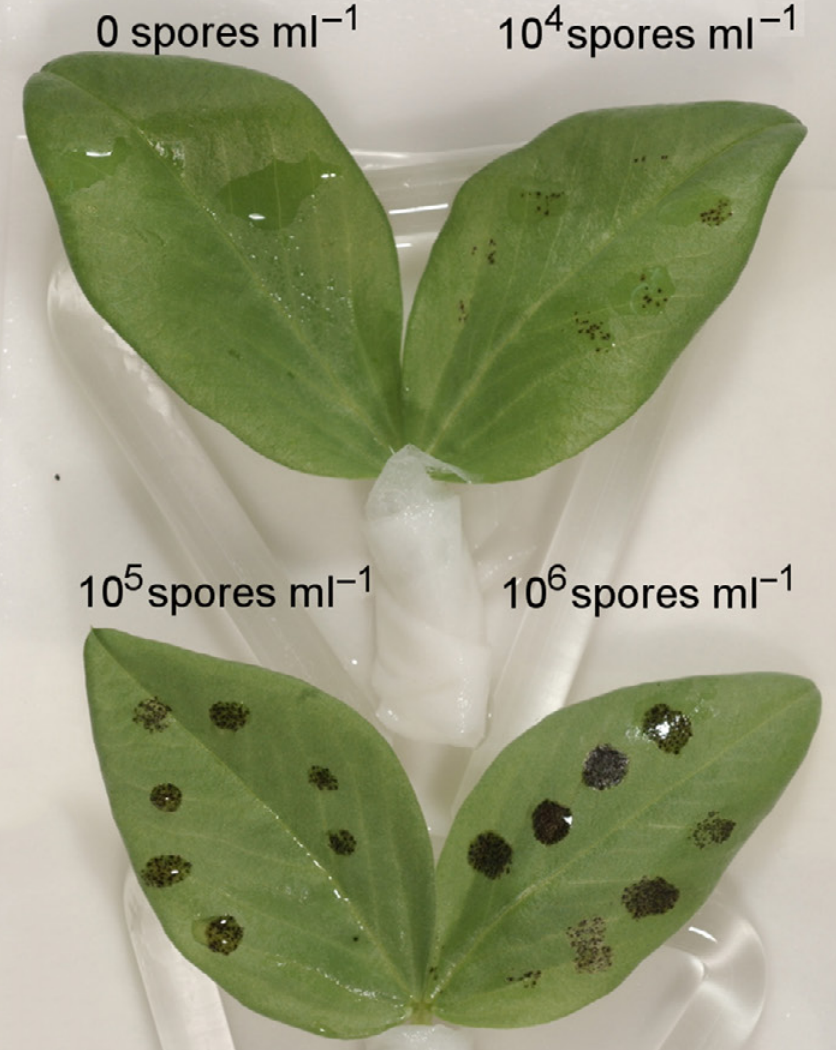
\includegraphics[width=0.8\linewidth]{../images/inoculum_potential} \caption{The inoculum potential (i.e. the amount of pathogen available) can influence success of colonisation, as illustrated here with different spore loads of the necrotrophic pathogen Botrytis cinerea added to the surface at eight points on broad bean (Vicia faba) leaves.}\label{fig:inoculum-potential}
\end{figure}

\ecolumns
\end{frame}

\begin{frame}{Preparation and application}
\protect\hypertarget{preparation-and-application}{}
\footnotesize

\textbf{Preparation (case with virus)}

\begin{itemize}
\tightlist
\item
  Select a part of the diseased plant in which the virus concentration
  is expected to be highest, such as young leaves showing clear symptoms
\item
  Leaf material is ground with water or 0.01 M phosphate buffer (less
  often borate, citrate or Tris buffer may be desirable), pH 7.0, in a
  tissue-to-maceration fluid ratio (w/v) of 1:5 to 1:10.
\item
  Often plant cell contain constituents ( Protein inhibitors in
  \emph{Chenopodiaceae} family, polyphenoloxidases in plant sap, tannins
  in plants of Rosaceae family) which inhibit infection, either by
  inactivating the virus or by decreasing the susceptibility of the test
  plant.
\end{itemize}
\end{frame}

\begin{frame}{}
\protect\hypertarget{section-1}{}
\begin{itemize}
\tightlist
\item
  If fruiting structures (pycnidia, perithecia) are present on the leaf,
  it is sometimes possible to pick them out, drop them in the surface
  sterilant for a few seconds, and then plate them on the nutrient
  medium. This requires use of stereoscopic microscope.
\item
  Structures may be crushed in a small drop of sterile water and then
  the spores in the water may be diluted serially in small tubes or
  dishes containing sterile water.
\end{itemize}

\begin{block}{}
\protect\hypertarget{section-2}{}
The serial dilution method is often used to isolate pathogenic bacteria
from diseased tissues contaminated with other bacteria. After surface
sterilization of sections of diseased tissues from the margin of the
infection, the sections are ground aseptically but thoroughly in a small
volume of sterile water and then part of the homogenate is diluted
serially in equal volumes or 10 times the volume of the initial water.

(\scriptsize Refer to the youtube video by Katharine Hubbard)
\end{block}
\end{frame}

\begin{frame}{Application of inoculum}
\protect\hypertarget{application-of-inoculum}{}
\small

\begin{itemize}
\tightlist
\item
  With soilborne pathogen, seed or root of seedlings is dipped in a
  spore suspension or inoculum or mix inoculum with the pot soil or
  apply with a pipette or syringe to the basis of each plant.
\item
  With pathogens like powdery mildew and rust, spray or dust the
  inoculum over the plants.
\item
  While applying virus inoculum, small wounds are made in plant itself
  to achieve infection. This can be achieved mechanically or by dusting
  with abrasives, e.g.~Carborundum powder. Dusted leaves are inoculated
  by rubbing their surface with the inoculum.
\item
  Rice is inoculated with \emph{Xanthomonas campestris} pv.
  \emph{oryzae} by clipping the leaf tips with a pair of scissors that
  are dipped in bacterium suspension and bacterium gets access to leaf
  tissue through the wound.
\item
  Field application must ensure that inoculum from polycyclic leaf
  pathogens reach to plants to be tested from the spreader rows,
  \(\therefore\) spreader rows are inoculated early in the season.
\end{itemize}
\end{frame}

\begin{frame}{}
\protect\hypertarget{section-3}{}
\textbf{Method of inoculation in (case with virus)}

\bcolumns
\column{0.65\textwidth}
\small

\begin{itemize}
\tightlist
\item
  Common method is rubbing with the forefinger, foam plastic blocks,
  glass spatulae, and artist's paint-brush.
\item
  All these techniques may lead to satisfactory infection, provided they
  are able to create wounds small enough not to damage the cells too
  much and big enough to enable the virus particles to enter the cell.
\item
  Using disposable materials for inoculation avoids the requirement for
  washing of hands.
\item
  Use of glass spatulae is handy when many inocula in small amounts have
  to be prepared and applied, e.g., from a large number of single local
  lesions.
\item
  Inoculum is gently rubbed over the leaf (no more than twice on the
  same area) from its base to the top.
\end{itemize}

\column{0.35\textwidth}

\begin{center}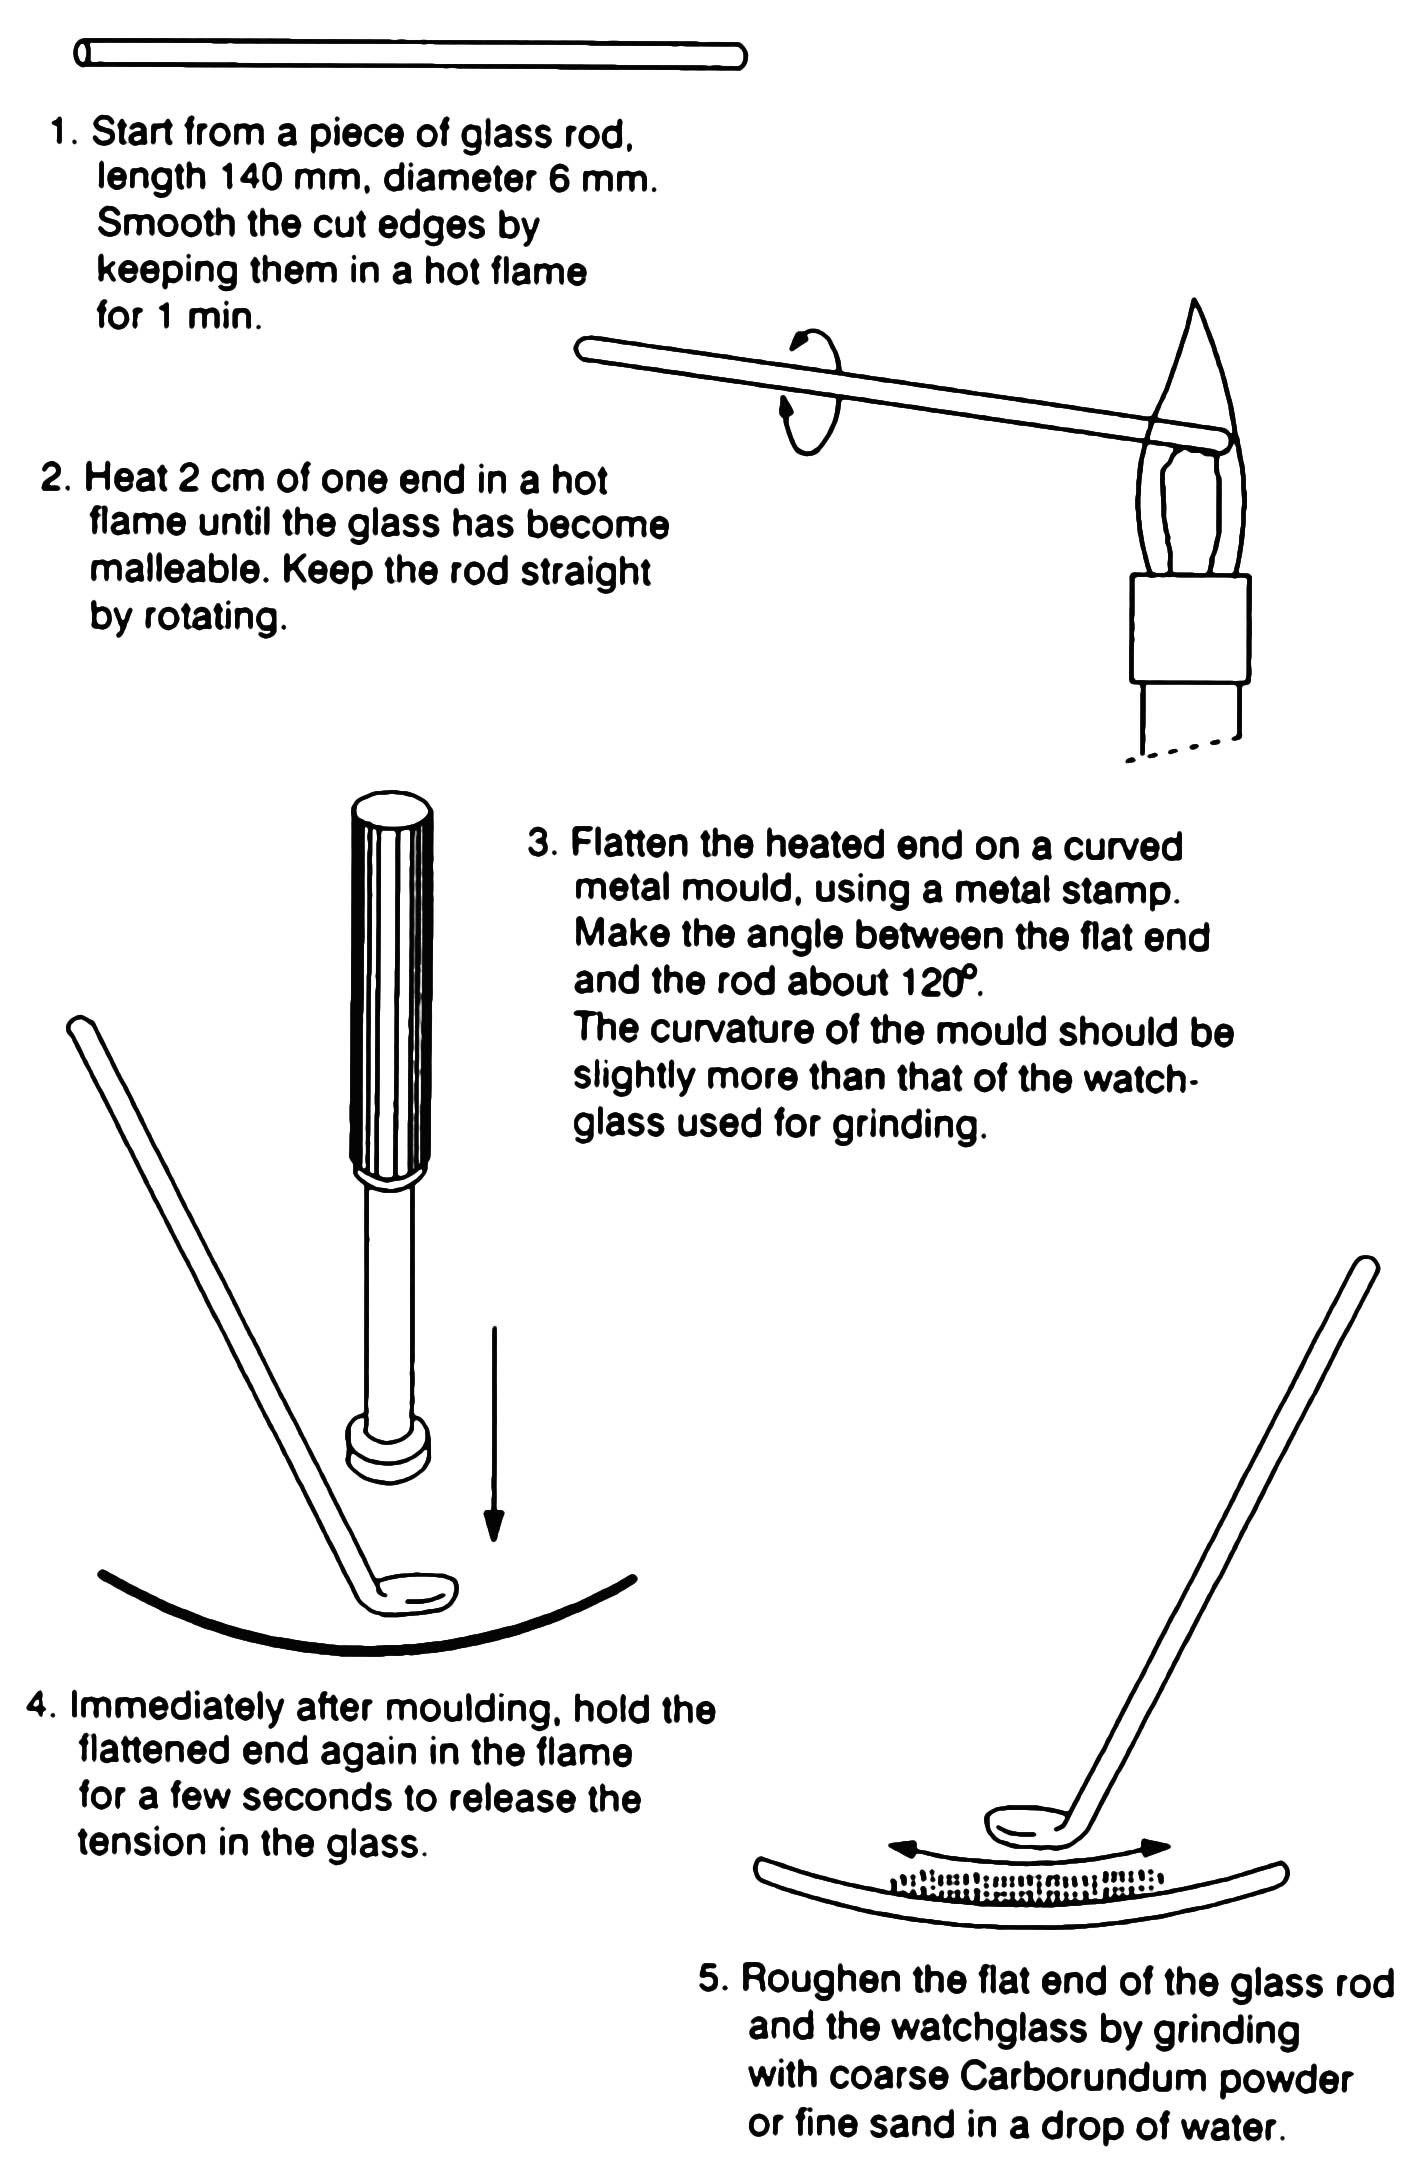
\includegraphics[width=0.76\linewidth]{../images/glass_spatula_for_mechanical_inoculation} \end{center}

\ecolumns
\end{frame}

\begin{frame}{Composing inoculum}
\protect\hypertarget{composing-inoculum}{}
\footnotesize

\begin{itemize}
\tightlist
\item
  In case or race-specific resistance results of the test depend very
  much on pathogen race that is applied, \(\therefore\) isolates need to
  be characterized to select for proper races
\item
  Steps

  \begin{itemize}
  \footnotesize
  \item Obtain a genetically homogeneous isolate
  \item Apply individual propagules of the pathogen on nutrient medium or on a susceptible plant
  \item Derive each sporulating colony or lesign from one single propagule (spore) that can be propagated in isolation to a genetically pure 'monospore isolate'
  \end{itemize}
\item
  One may expect many different genes for race-specific resistance in
  some plant-pathosystems. In such case in order to detect new gene that
  provide complete resistance test will be carried out with the most
  complex race available or with a mixture of isolates.
\item
  In partial resistance and application of a mixture of isolates, one
  may find differences in amount of infection among the germplasm and
  interpret results as,

  \begin{itemize}
  \footnotesize
  \item being caused by difference in level of race non-specific resistance against these isolates
  \item tested plants differ in genes for complete, race-specific resistance that is effective against one or more of the isolates in the mixture
  \end{itemize}
\end{itemize}
\end{frame}

\begin{frame}{Handling of test plants}
\protect\hypertarget{handling-of-test-plants}{}
\small

\begin{itemize}
\tightlist
\item
  Plant species/cultivars of the families Amaranthaceae, Chenopodiaceae,
  Cucurbitaceae, Leguminosae and Solanaceae are known to be easily
  infected by a large number of viruses. Usually a selection of a number
  of test plant species from these families is made to study the host
  range of an unidentified virus.
\item
  Susceptibility of a test plant depends on a number of factors, such as

  \begin{itemize}
  \item genotype (to account for differences always grow replicates of test plants), 
  \item physiological condition determined by temperature,
  \item light intensity and humidity, under which it has been raised,
  \item nutrition,
  \item age
  \end{itemize}
\item
  Leaves of young well-nurished plants grown rapidly in moderate light
  conditions and usually the most susceptible
\item
  Primary leaves of \emph{Phaseolus} spp. and \emph{Vigna} spp. are more
  suceptible compared to their trifoliate leaves.
\item
  Period of darkening of the plants for 1-2 days prior to inoculation
  leads to \(\uparrow\) infection rate.
\end{itemize}
\end{frame}

\hypertarget{natural-reserves-of-disease-inoculum}{%
\section{Natural reserves of disease
inoculum}\label{natural-reserves-of-disease-inoculum}}

\begin{frame}{Fungi}
\protect\hypertarget{fungi}{}
\small

\begin{itemize}
\tightlist
\item
  In Zygomycetes ( \emph{Rhizopus} spp., \emph{Mucor} spp.),
  sporangiospores float about if they land on wounds of fleshy fruits,
  roots, corms and bulbs thoughout the year.

  \begin{itemize}
  \tightlist
  \item
    Fungal mycelium does not invade cells but is instead surrounded by
    dead cells and non-living organic substances
  \item
    Once fungus establishes in ``soft tissue'' (owing to the nature of
    damage it inflicts from secretion of pectinolytic enzymes), it
    emerges through wounds producing aerial sporangiophores/sporangia.
  \item
    When food supply in the infected tissues diminish and compatible
    strains are present together, zygospores are produced which survive
    periods of starvation and adverse temperature/moisture.
  \end{itemize}
\item
  In Ascomycetes fungi, overwintering structure such as mycelium or even
  spores serve as inoculum for the disease development the following
  season (spring and summer).

  \begin{itemize}
  \tightlist
  \item
    In Powdery mildew of roses (caused by \emph{Sphaerotheca pannosa}),
    shoots arising from buds containing mycelium or
    cleistothecia/ascocarp (which produce ascospores) become infected
    and provide inoculum for secondary infection and disease development
    on foliage and flowers.
  \end{itemize}
\end{itemize}
\end{frame}

\begin{frame}{}
\protect\hypertarget{section-4}{}
\small

\begin{itemize}
\tightlist
\item
  \ldots{}

  \begin{itemize}
  \footnotesize
  \item Diseases caused by \textit{Alternaria} appear usually as leaf spots and blights (while also causing damping-off, stem rots, tuber/fruit rot) and the major infectious factor (primary inoculum) is the spore -- conidia (present in air and dust). Many species of this genera are saprophytic.
  \item \textit{Colletotrichum} spp. (Anthracnose of fruit, root rot and crown rot of developing plant), \textit{Cochliobolus miyabeanus} (Brown spot in rice), \textit{Pyrenophora} spp. (Net blotch of barley, Tan spot of wheat) groups of mitosporic fungi overwinter in or on infected or contaminated seeds, in plant debris of susceptible plants
  \item \textit{Monilinia} spp. overwinter as mycelium in mummified fruit on the tree and in the cankers of affected twigs or as pseudosclerotia above-ground which prduce new conidia in the spring. Pseudosclerotia buried in the ground produce apothecia, which form asci and ascospores.
  \item \textit{Fusarium} spp. (causing vascular wilt) survives in infected plants as mycelium and in soil debris it forms chlamydospores (most commonly in colder temperature) which are transported through water and contaminated equipments.
  \item Fusarium (Gibberella) head blight of cereals is more severe in warm, humid weather, wherein pinkish-red mycelium and conidia develop abundantly in the infected spikelets, and the infection spreads to adjacent spikelets or through the entire head. Purplish perithecia may also develop on the infected floral bracts. Infected kernels become shriveled and discolored with a white, pink, or light-brown scaly appearance as a result of the mycelial outgrowths from the pericarp.
  \end{itemize}
\end{itemize}
\end{frame}

\begin{frame}{Screening for Fusarium wilt resistance}
\protect\hypertarget{screening-for-fusarium-wilt-resistance}{}
\begin{itemize}
\tightlist
\item
  Done multiple times in a year
\item
  Innoculation suspension
\end{itemize}
\end{frame}

\begin{frame}{Cautions about field inoculation study}
\protect\hypertarget{cautions-about-field-inoculation-study}{}
\begin{itemize}
\tightlist
\item
  Screening methods are time taking, laborious and require larger area.
\item
  The field inoculation techniques are inherently poor in terms of
  reproducibility as a result of uneven inoculum distribution,
  interaction with other pathogens, and variations in weather and other
  environmental factors which may affect disease severity.
\end{itemize}
\end{frame}

\hypertarget{evaluation-aspects-quantitative-and-qualitative-aspects}{%
\section{Evaluation aspects: Quantitative and Qualitative
aspects}\label{evaluation-aspects-quantitative-and-qualitative-aspects}}

\begin{frame}{Dilution test}
\protect\hypertarget{dilution-test}{}
\begin{itemize}
\tightlist
\item
  Agar dilution is a method used to determine the Minimum Inhibitory
  Concentration (MIC) of antibiotics.
\item
  Method is useful when the effectiveness of a new antibiotic (among a
  few available antibiotics) is to be tested against a large panel of
  bacteria.
\item
  Antibiotic is diluted with water to produce a series of concentrations
\end{itemize}
\end{frame}

\begin{frame}{Measurement of field infection (visual scoring)}
\protect\hypertarget{measurement-of-field-infection-visual-scoring}{}
\footnotesize

\begin{itemize}
\tightlist
\item
  Amount of infection by polycyclic leaf pathogen is usually assessed by
  estimating the percentage of leaf tissue covered with lesions,
  mycelium or pustules.
\item
  When such observations are repeated several times in the season on the
  same plant or field plots, an impression is obtained of the increase
  of the infection over time.
\item
  The idea also forms basis for disease epidemiology and disease
  forcasting as it leads to formulation of model for a particular
  disease.
\item
  `Area Under the Disease Progress Curve' (AUDPC) can be calculated from
  the graph in which the amount of infection recorded is plotted against
  the time during which it occured.
\end{itemize}

\begin{equation}
AUDPC = \sum_{i = 1}^a \left [\left\{ \frac{Y_i + Y_{(i+1)}}{2}\right\} \times (t_{(i+1)}-t_i)\right ]
\end{equation}

\begin{itemize}
\tightlist
\item
  Where,

  \begin{itemize}
  \footnotesize
  \item $Y_i$ is the disease score at the time $t_i$
  \item $t_{(i+1)}-t_i$ is the duration (in days) between recording of two scores for the same unit
  \end{itemize}
\end{itemize}
\end{frame}

\begin{frame}{}
\protect\hypertarget{section-5}{}
\begin{figure}
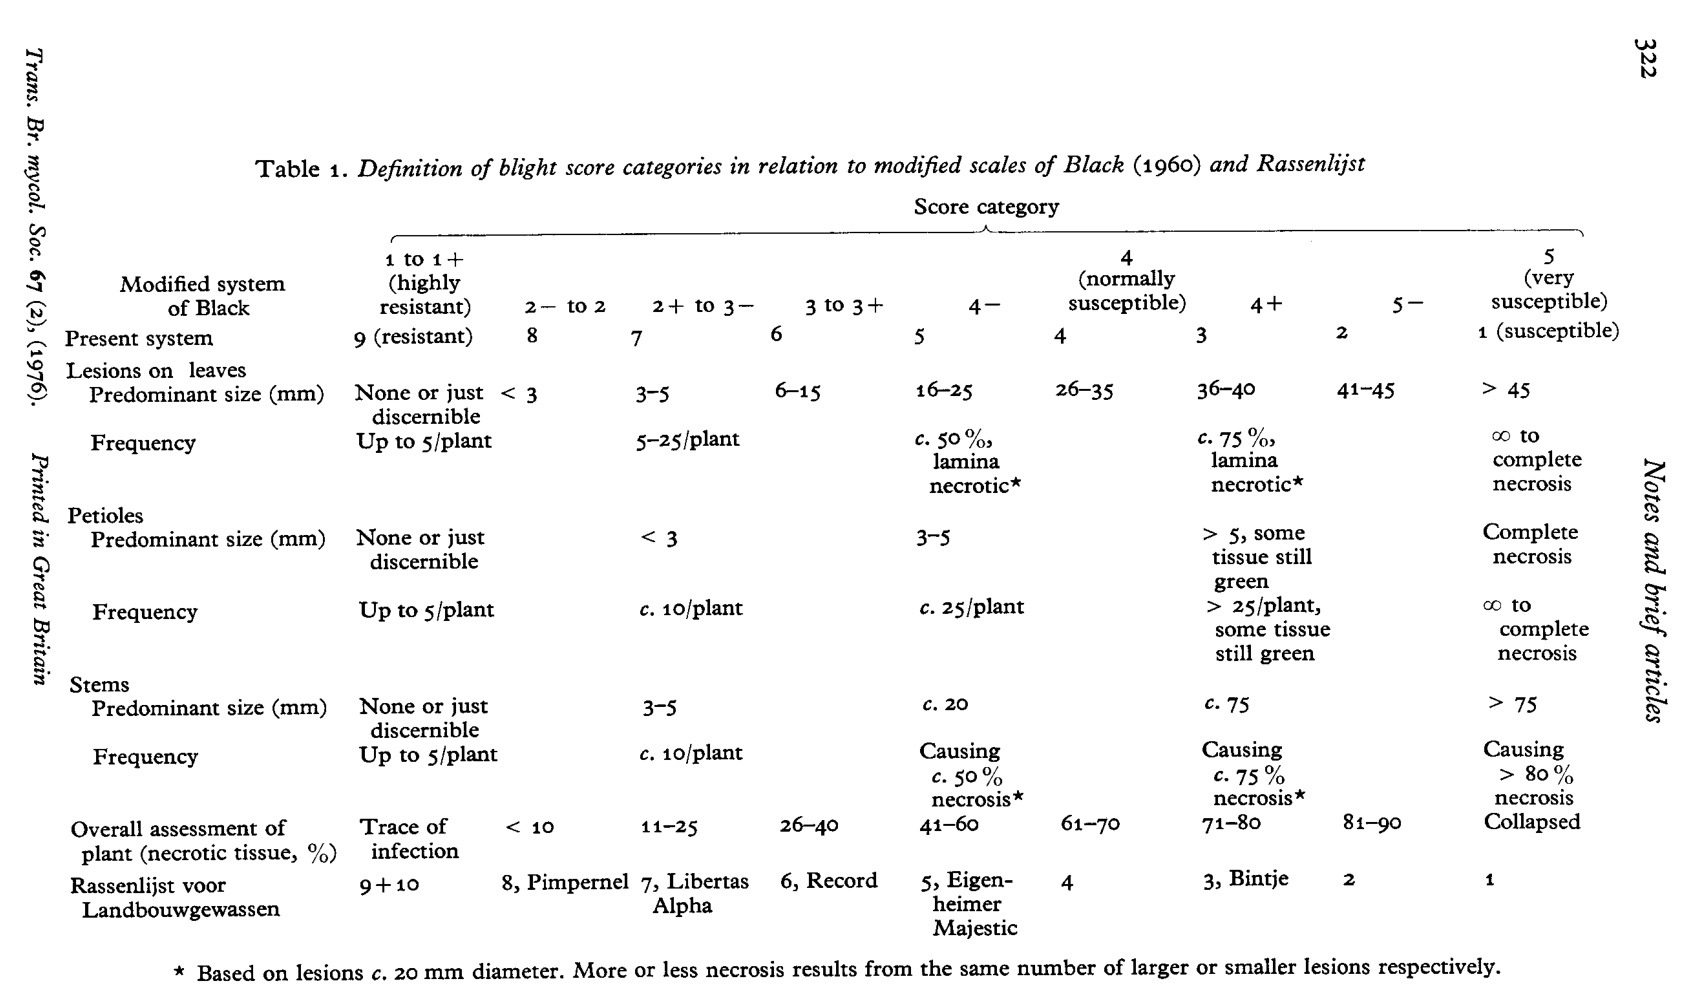
\includegraphics[width=0.8\linewidth]{../images/phytophthora_infestans_infection_assessment} \caption{Disease assessment by visual scoring, a case of potato late blight. Source: \cite{malcolmson1976assessment}.}\label{fig:phytophthora-infection-assessment}
\end{figure}
\end{frame}

\begin{frame}{}
\protect\hypertarget{section-6}{}
\begin{figure}
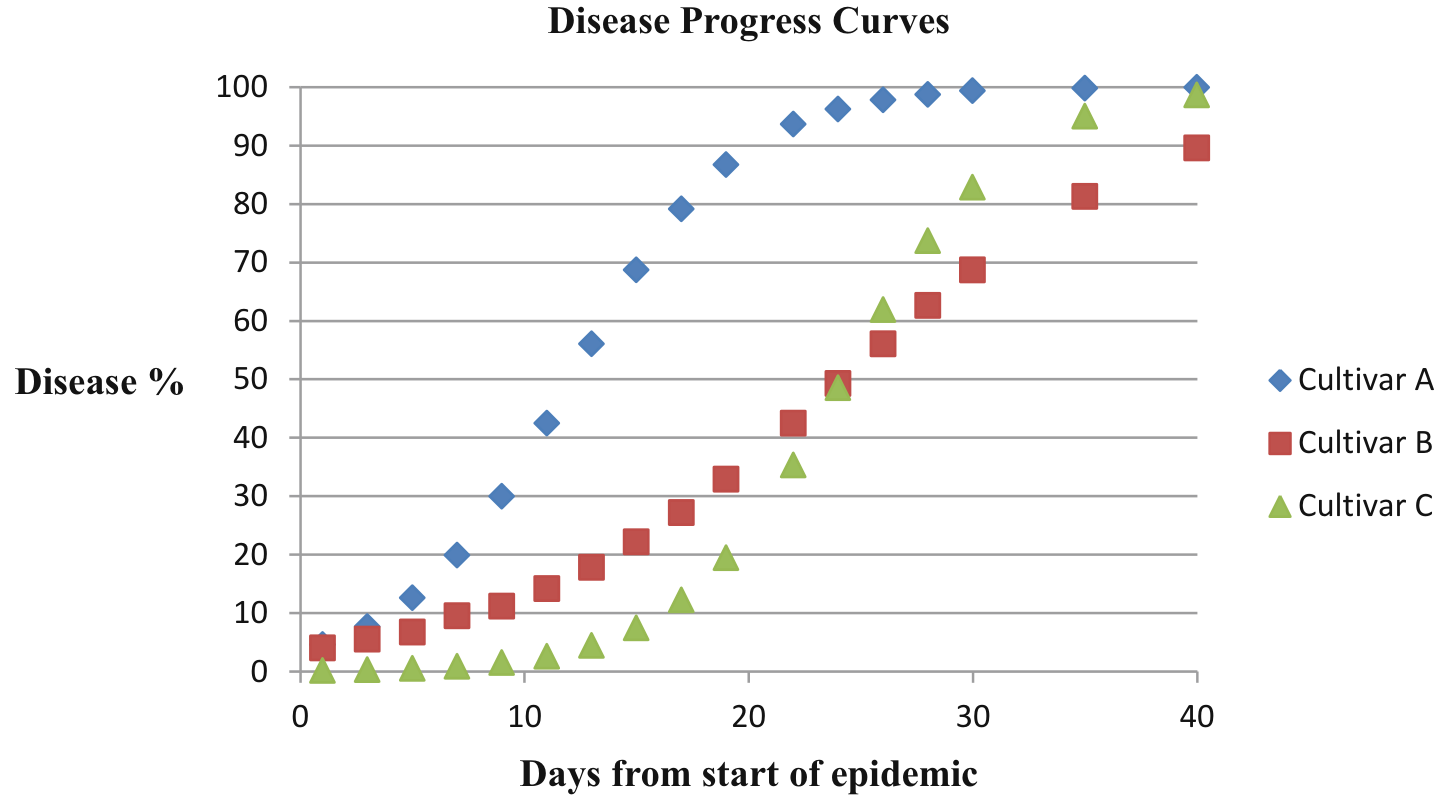
\includegraphics[width=0.8\linewidth]{../images/audpc_curve_john_bradshaw} \caption{Theoretical disease progress curves differing in infection rate ($r$) and intercept ($k$) (cultivar A: r = 0.2725 and k = -3.299; cultivar B: r = 0.13625 and k = -3.299; cultivar C: r = 0.2725 and k = -6.598).}\label{fig:audpc-theoretical}
\end{figure}
\end{frame}

\hypertarget{bibliography}{%
\section{Bibliography}\label{bibliography}}

\begin{frame}{References}
\protect\hypertarget{references}{}
\end{frame}

          \begin{frame}[allowframebreaks]{}
    \bibliographytrue
    \bibliography{./../bibliographies.bib}
    \end{frame}
  


\end{document}
